% chapter 1 section 3

\section{特殊运动}

\paragraph{惯性力}为非惯性系\footnote{系统参照物做非等速直线运动的系}下维持平衡的力,在部分情形下会使问题分析变得简单。
\begin{figure}[ht!]
    \centering
    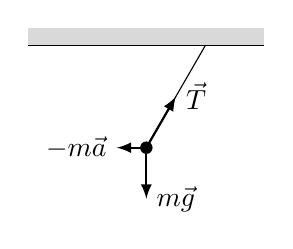
\begin{tikzpicture}[scale=0.75]
        \draw (-1, 0) -- (3, 0);
        \fill[fill=gray, opacity=0.3] (-1, 0) rectangle (3, 0.3);
        \draw (2, 0) -- (1, {-sqrt(3)});
        \fill (1, {-sqrt(3)}) circle (3pt);
        \draw[thick, -latex] (1, {-sqrt(3)}) -- ++ (-0.5, 0) node[left] {$-m\vec{a}$};
        \draw[thick, -latex] (1, {-sqrt(3)}) -- ++ (0.5, {0.5*sqrt(3)}) node[right] {$\vec{T}$};
        \draw[thick, -latex] (1, {-sqrt(3)}) -- ++ (0, {-0.5*sqrt(3)}) node[right] {$m\vec{g}$};
    \end{tikzpicture}
    \caption{非惯性系}
\end{figure}

\subsection{圆周运动}

\subsubsection{等速圆周运动}

\begin{figure}[ht!]
    \centering
    \begin{minipage}[t]{0.48\textwidth}
        \centering
        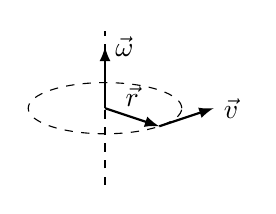
\begin{tikzpicture}[scale=0.65]
            \draw[dashed] (0, -1.5) -- (0, 1.5);
            \draw[thick, -latex] (0, 0) -- (0, 1.2) node[right] {$\vec{\omega}$};
            \draw[dashed] (0,0) circle (1.5 and 0.5);
            \draw[thick, -latex] (0, 0) -- node[above] {$\vec{r}$} (-45:1.5 and 0.5);
            \draw[thick, -latex] (-45:1.5 and 0.5) -- ++ (45:1.5 and 0.5) node[right] {$\vec{v}$};
        \end{tikzpicture}
        \caption{角速度}
    \end{minipage}
    \begin{minipage}[t]{0.48\textwidth}
        \centering
        \begin{tikzpicture}[scale=0.65]
            \draw (0, 0) circle (1.5) node[below] {$O$};
            \draw (1.5, 0) -- (0, 0) -- node[above] {$r$} (45:1.5) node[right] {$(r\cos\omega t, r\sin\omega t)$};
            \drawangle[$\omega t$]{(1, 0)}{(0, 0)}{(45:1)};
            \draw[thick, -latex] (45:1.5) -- node[right] {$v$} ++ ($0.6*(135:1.5)$);
        \end{tikzpicture}
        \caption{圆周运动加速度}
    \end{minipage}
\end{figure}
\begin{itembox}[l]{角速度与周期}
    \begin{equation*}
        \omega = \frac{d\theta}{dt}
    \end{equation*}
    \begin{itemize}
        \item 单位:$rad/s$
        \item 线速度:$v=\omega r$
        \item 周期:$T=\frac{2\pi}{\omega}$
    \end{itemize}
\end{itembox}
作为对圆周运动方式的本质描述,角速度是同时具有方向与大小的矢量,其标准定义为:$\vec{\omega}=\frac1{r^2}\vec{r}\times\vec{v}$。
\begin{itembox}[l]{圆周运动加速度}
    \begin{itemize}
        \item 大小:
        \begin{equation*}
            a=\omega^2r=\frac{v^2}{r}
        \end{equation*}
        \item 方向:指向圆心
    \end{itemize}
\end{itembox}

\paragraph{向心力}物体做圆周运动的过程中时时刻刻都在改变着运动状态,那么实现这个改变的力便是\underline{向心力}。同时在生活中也常常使用离心力一词,在物理中也同样存在这个说法,其与向心力的区别在于观察角度的不同。
\begin{itemize}
    \item 向心力:是惯性系下观察时维持圆周运动的合外力
    \item 离心力:日文为遠心力,是非惯性系下观察时是物体保持静止的力
\end{itemize}
事实上,解决圆周问题的核心就在于发现是什么力构成了向心力。

\paragraph{圆锥摆}日文为円すい振り子,是一种简单常见的平面圆周运动模型。
\begin{figure}[ht!]
    \centering
    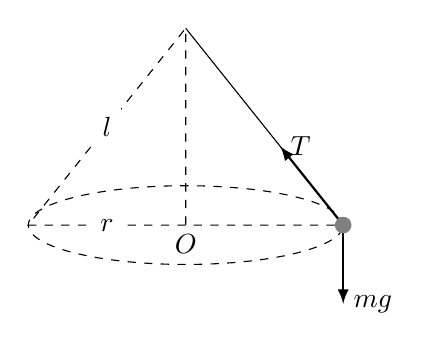
\begin{tikzpicture}
        \begin{scope}[yscale=0.25]
            \draw[dashed] (0, 0) circle (2);
        \end{scope}
        \draw[dashed] (0, 0) -- node[fill=white] {$r$} (-2, 0) -- node[fill=white] {$l$} (0, 2.5) -- (0, 0) node[below] {$O$} -- (2, 0);
        \draw (2, 0) -- (0, 2.5);
        \drawangle{(0, 0)}{(0, 2.5)}{(2, 0)};
        \draw[thick, -latex] (2, 0) -- ++ (-0.8, 1) node[right] {$T$};
        \draw[thick, -latex] (2, 0) -- ++ (0, -1) node[right] {$mg$};
        \fill[fill=gray] (2, 0) circle (3pt);
    \end{tikzpicture}
    \caption{圆锥摆}
\end{figure}
受力分析后可知,水平方向上$T\sin\theta=F_\textrm{向}$,竖直方向上$T\cos\theta=mg$。联立可解角速度大小。
\begin{equation*}
    \omega=\sqrt{\frac{g}{l\cos\theta}}
\end{equation*}

\subsubsection{非等速圆周运动}

\paragraph{绳线模型}接下来考虑如下模型:竖直平面内一个由线牵引的小球的运动。
\begin{figure}[ht!]
    \centering
    \begin{tikzpicture}
        \draw (0, -4) -- node[fill=white] {$r$} (0, 0) -- (-45:4);
        \draw[dashed] (-90:4) arc (-90:-20:4);
        \drawangle{(0, -4)}{(0, 0)}{(-45:4)};
        \draw[dashed] (0, -4) -- (-2, -4);
        \draw[dashed] (-45:4) -- (-2, {-2*sqrt(2)});
        \draw[<->] (-1.8, -4) -- node[fill=white] {$r(1-\cos\theta)$} (-1.8, {-2*sqrt(2)});
        \draw[thick, -latex] (0, -4) -- node[below] {$v_0$} ++ (1, 0);
        \fill[gray] (0, -4) circle (3pt);
        \draw[thick, -latex] (-45:4) -- node[right] {$v$} ++ ($0.5*(45:2)$);
        \draw[thick, -latex] (-45:4) -- node[above] {$T$} ++ ($0.8*(135:2)$);
        \draw[thick, -latex] (-45:4) -- ++ (0, -1) node[below] {$mg$};
        \fill[gray] (-45:4) circle (3pt);
    \end{tikzpicture}
    \caption{竖直平面圆周运动}
\end{figure}
将合力/加速度在平行和垂直运动方向上分解后可发现,垂直于运动方向的部分只负责维持各个瞬间的圆周运动,而平行于运动方向的部分只负责调整速度。此外,运动的物体只受重力(保存力)和绳子的拉力,而拉力时时刻刻又与运动方向垂直(不做功),所以整个系统机械能守恒。

\subparagraph{拉力大小}
\begin{align*}
    T=&G\cos\theta+m\frac{v^2}{r}\\
    \downarrow&\quad\frac12m{v_0}^2=\frac12mv^2+mgr(1-\cos\theta)\\
    =&mg\cos\theta+\frac{m{v_0}^2}{r}-2mg(1-\cos\theta)\\
    =&\frac{m{v_0}^2}{r}+mg(3\cos\theta-2)
\end{align*}

\subparagraph{最小初速度}
\begin{equation*}
    \begin{cases}
        \frac12m{v_0}^2=\frac12mv^2+2mgr\\
        mg=m\frac {v^2}r
    \end{cases}
    \implies v_{min}=v_0=\sqrt{5gr}
\end{equation*}

\paragraph{其他变形}在实际题目中除了用绳线做牵引,还有一些其他相似模型。
\begin{figure}[ht!]
    \centering
    \renewcommand\arraystretch{1.2}
    \begin{tabular}{c|cc}
        \hline
        牵引物&半周前&半周后\\\hline
        线/圆筒面&拉力&无\\
        棒/管内&拉力&支持力\\\hline
    \end{tabular}
    \caption{非等速圆周运动模型}
\end{figure}

\subsection{简谐振动}

\subsubsection{基本概念}

首先考虑如下模型:物体在平面上做等速圆周运动,其一侧有光源,另一侧有一光屏,观察光屏上点的运动模式。
\begin{figure}[ht!]
    \centering
    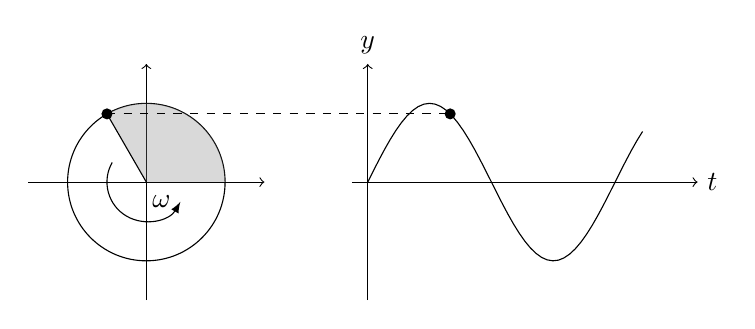
\begin{tikzpicture}
        \begin{scope}[xshift=-80]
            \draw[->] (-1.5, 0) -- (1.5, 0);
            \draw[->] (0, -1.5) -- (0, 1.5);
            \draw (0, 0) circle (1);
            \fill[fill=gray, opacity=0.3] (0, 0) -- (1, 0) arc (0 : 120 : 1) --cycle;
            \coordinate (P) at (120 : 1);
            \fill (P) circle (2pt);
            \draw (0, 0) -- (P);
            \draw[-latex] (150:0.5) arc (150:330:0.5) node[left] {$\omega$};
        \end{scope}
        \begin{scope}
            \draw[->] (-0.2, 0) -- ({rad(240)}, 0) node[right] {$t$};
            \draw[->] (0, -1.5) -- (0, 1.5) node[above] {$y$};
            \draw[domain=0:rad(200)] plot[samples=50] (\x, {sin(2*\x r)});
            \coordinate (Q) at ({rad(60)}, {sin(60)});
            \fill (Q) circle (2pt);
        \end{scope}
        \draw[dashed] (P) -- (Q);
    \end{tikzpicture}
    \caption{简谐振动}
\end{figure}
可见该点的位置(y坐标)与时间呈三角函数关系。这种物理量与时间呈三角函数关系的运动即为\underline{简谐振动},日文为単振動。其运动学信息可由等速圆周运动轻松求得。
\begin{itembox}[l]{简谐振动的运动学信息}
    \begin{itemize}
        \item 位移:$x=A\sin(\omega t+\theta_0)$
        \item 速度:$v=A\omega\cos(\omega t+\theta_0)$
        \item 加速度:$a=-A\omega^2\sin(\omega t+\theta_0)=-\omega^2x$
    \end{itemize}
\end{itembox}

\subsubsection{回复力}

结合牛二定律可见,做简谐振动的物体始终都会受到一个与位移方向相反的力,名为\underline{回复力},日文为復元力。因为位移的方向是以振动中心为基准向外的,所以回复力的方向即是始终指向其振动中心。
\begin{itembox}[l]{回复力}
    \begin{equation*}
        F=ma=-m\omega^2x=-kx\quad(k=m\omega^2)
    \end{equation*}
    \begin{itemize}
        \item $F\propto x$
        \item 方向指向振动中心
    \end{itemize}
\end{itembox}
此外,回复力的数学形式与弹簧弹力相像,所以不难推断回复力做功也与路径无关,属于保存力。因此简谐振动也满足机械能守恒。

虽然简谐振动中角速度不存在实际意义,但利用$T=\frac{2\pi}{\omega}$的关系,我们就可以得到简谐振动的周期。
\begin{itembox}[l]{简谐振动周期}
    \begin{equation*}
        T=2\pi\sqrt{\frac{m}{k}}
    \end{equation*}
\end{itembox}

\subsubsection{弹簧振子}

日文为バネ振り子,是最常见的简谐振动模型。
\begin{figure}[ht!]
    \centering
    \begin{tikzpicture}
        \begin{scope}
            \draw (0, 0) -- (5, 0);
            \fill[fill=gray, opacity=0.3] (0, 0) rectangle (5, -0.3);
            \draw (0.2, 0) -- (0.2, 0.5);
            \draw[spring] (0.2, 0.25) -- ++ (3.2, 0);
            \draw[fill=white] (3.5, 0.25) circle (6pt);
            \draw[-latex, rounded corners=2pt] (3.5, 1) -- (5, 1) -- (5, 0.9) -- (2, 0.9) -- (2, 0.8) -- (3.5, 0.8);
        \end{scope}
        \begin{scope}[xshift=200, yshift=50]
            \draw (0, 0) -- (3, 0);
            \fill[fill=gray, opacity=0.3] (0, 0) rectangle (3, 0.3);
            \draw[spring] (1, 0) -- ++ (0, -2);
            \draw[spring] (2, 0) -- ++ (0, -2.3);
            \draw[fill=white] (2, -2.5) circle (6pt);
            \draw[-latex, rounded corners=2pt] (2.3, -2.5) -- (2.3, -4) -- (2.4, -4) -- (2.4, -1) -- (2.5, -1) -- (2.5, -2.5);
        \end{scope}
    \end{tikzpicture}
    \caption{弹簧振子}
\end{figure}
对于水平放置的弹簧,其回复力就是弹簧弹力,振动中心为原长处。对于竖直放置的情况受力分析后,可列如下等式。
\begin{align*}
    F=&mg-kx\\
    \downarrow&\quad mg=kx_0\\
    =&-k(x-x_0)
\end{align*}
即回复力中的k值仍旧是弹簧的弹性系数,振动中心下移至了平衡位置。更一般的,对于任意形式放置的弹簧上述结论皆成立。

\subsubsection{单摆}

日文为単振り子,属于摆动幅度极小的竖直平面圆周运动的模型。
\begin{figure}[ht!]
    \centering
    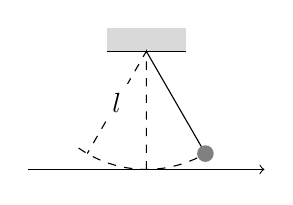
\begin{tikzpicture}
        \draw (-0.5, 0) -- (0.5, 0);
        \fill[fill=gray, opacity=0.3] (-0.5, 0) rectangle (0.5, 0.3);
        \draw[->] (-1.5, -1.5) -- (1.5, -1.5);
        \draw[dashed] (-125:1.5) arc (-125:-55:1.5);
        \draw (-60:1.5) -- (0, 0);
        \draw[dashed] (-90:1.5) -- (0, 0) -- node[fill=white] {$l$} (-120:1.5);
        \drawangle{(-90:1.5)}{(0, 0)}{(-60:1.5)};
        \fill[fill=gray] (-60:1.5) circle (3pt);
    \end{tikzpicture}
    \caption{单摆}
\end{figure}
鉴于其周期推导略复杂,这里直接给出结论。
\begin{itembox}[l]{单摆周期公式}
    \begin{equation*}
        T=2\pi\sqrt{\frac{l}{g}}
    \end{equation*}
\end{itembox}

\subsection{天体运动}

\subsubsection{开普勒定律}

开普勒定律是开普勒基于其老师第谷的实验数据总结而得的。而且此定律不仅适用于恒星与其行星之间,行星与其卫星也同样适用。
\begin{itembox}[l]{开普勒定律}
    \begin{itemize}
        \item 轨道法则:行星运动在以恒星为焦点的椭圆轨道上
        \item 面积法则:行星与恒星连线的$\begin{cases}\textrm{在单位时间内扫过的面积}\\\textrm{面积速度}\end{cases}$相等
        \item 周期法则:$T^2=ka^3\quad(k:const)$
    \end{itemize}
\end{itembox}
\begin{figure}[ht!]
    \centering
    \begin{tikzpicture}
        \fill ({-sqrt(5)}, 0) circle (1.5pt);
        \draw (0, 0) circle (3 and 2);
        \draw ({-sqrt(5)}, 0) -- node[fill=white] {$r$} ++ ($({sqrt(5)}, 0)+(10:3 and 2)$);
        \draw ({-sqrt(5)}, 0) -- ++ ($({sqrt(5)}, 0)+(30:3 and 2)$);
        \draw[thick, -latex] (10:3 and 2) -- ++ (-0.3, 1) node[right] {$v$};
        \drawangle{($(10:3 and 2)+(-0.3, 1)$)}{(10:3 and 2)}{(0, 0)};
    \end{tikzpicture}
    \caption{面积速度}
\end{figure}
\begin{itembox}[l]{面积速度}
    \begin{equation*}
        \frac{dS}{dt}=\frac{\frac12r(v\cdot dt\sin\theta)}{dt}=\frac12rv\sin\theta
    \end{equation*}
\end{itembox}

\subsubsection{万有引力定律}

\paragraph{万有引力}是牛顿根据开普勒第三定律的思想发展出来的,描述物体间引力的理论。
\begin{itembox}[l]{万有引力公式}
    \begin{equation*}
        F=G\frac{m_1m_2}{r^2}\quad(\textrm{万有引力定数:}G=6.67\times10^{-11}N\cdot m^2\cdot kg^{-2})
    \end{equation*}
\end{itembox}
在实际运算过程中,一般将地表附近的万有引力视为重力。
\begin{itembox}[l]{黄金代换式}
    \begin{equation*}
        G\frac{Mm}{R^2}=mg\implies
        GM=gR^2
    \end{equation*}
\end{itembox}
但严格意义上讲,由于地球自转,地表上的物体还会受到离心力(非惯性系)。因此,实际的g值会比黄金代换式求得的值小一些。
\begin{figure}[ht!]
    \centering
    \begin{tikzpicture}[scale=0.8]
        \fill (0, 0) circle (1.5pt);
        \draw (0, 0) circle (2);
        \draw[thick, -latex] (45:2) -- (45:1) node[left] {万有引力};
        \draw[thick, -latex] (45:2) -- ($(45:2)+(0.5,0)$) node[right] {离心力};
        \draw[thick, -latex] (45:2) -- ($(45:1)+(0.5,0)$) node[below] {重力};
    \end{tikzpicture}
    \caption{万有引力与重力}
\end{figure}

\paragraph{万有引力势能}与重力类似,万有引力也有其对应的势能,为方便运算一般取无限远处为势能基准点。
\begin{figure}[ht!]
    \centering
    \begin{tikzpicture}[scale=0.8]
        \filldraw[color=black, fill=gray, fill opacity=0.3] (-30:1.5) arc (-30:210:1.5);
        \draw (-4, 0) -- (2, 0);
        \draw[->] (0, 0) -- (0, 4) node[right] {正};
        \draw[dashed] (0, 4) -- (-3, 4);
        \draw[<->] (-3, 0) -- node[fill=white] {$\infty$} (-3, 4);
        \draw[dashed] (0, 3) -- (-2, 3);
        \draw[<->] (-2, 0) -- node[fill=white] {$r$} (-2, 3);
        \draw[thick, -latex] (0, 3) -- node[right] {万有引力} (0, 2);
        \fill[fill=gray, opacity=0.5] (0, 3) circle (5pt);
    \end{tikzpicture}
    \caption{万有引力势能}
\end{figure}
\begin{itembox}[l]{万有引力势能(万有引力による位置エネルギー)}
    \begin{equation*}
        E_p=-G\frac{Mm}{r}
    \end{equation*}
\end{itembox}

\paragraph{应用}基于万有引力和万有引力势能即可试求两个宇宙速度。
\begin{figure}[ht!]
    \centering
    \begin{tikzpicture}
        \fill[fill=gray, opacity=0.3] (0, 0) circle (1.2);
        \draw[thick, -latex] (90:1.4) arc (90:-260:1.4) node[left, above] {第一宇宙速度};
        \draw[thick, -latex] (90:1.4) arc (90:0:2 and 3) node[right] {第二宇宙速度};
    \end{tikzpicture}
    \caption{宇宙速度}
\end{figure}

\subparagraph{第一宇宙速度}能够围绕地球旋转的最小速度。
\begin{equation*}
    m\frac{v^2}{r}=G\frac{Mm}{r^2}\implies
    v=\sqrt{gr}
\end{equation*}

\subparagraph{第二宇宙速度}能够挣脱地球引力的最小速度。
\begin{equation*}
    \frac12mv^2-G\frac{Mm}{r}=0(E_k)+0(E_p)\implies
    v=\sqrt{2gr}
\end{equation*}
